

\section{CV-VTON+} \label{section:cpvton+}

\subsection{Overview} 

Fig. 4 illustrates the new pipeline emphasizing the modifications from CP-VTON, which tackles all 4 issues above mentioned except extreme 3D pose of target human.

\begin{itemize}

\item Correction on the cloth agnostic representation   


\begin{itemize}

\item Modification 1: We added a new label ‘Skin’ to the human parsing data to represent the human body shape more accurately (Fig. 2. (a) right).

\item Modification 2: We removed the hair label from the Reserved Regions of GMM’s Person Representation input, i.e. only face remains.  

\end{itemize}


\item Un-changed human area inclusion  

\begin{itemize}
\item Modification 3: We added extra human components except the target cloth area, e.g. bottom clothes and legs in the Reserved Regions of Person Representation to TOM, along with face and hair (Fig. 2. (b) right).

\end{itemize}

\item Improving Composition alpha-map 


\begin{itemize}

\item Modification 4: In the mask loss term in TOM loss function, we replaced the Composition Mask with supervised ground truth mask for a strong alpha mask.

\begin{equation}
L=c_1 |I_0-I_{GT} |+  c_2 L_{VGG}+c_1 |M_{GT}-M_0 |       
\end{equation}

\item Modification 5: Lastly, we added the binary mask of warped cloth to TOM network input so that TOM can clearly differentiate the target cloth area regardless of cloth color.  

\end{itemize}

\item GMM improvement Will be here: GIC loss and Mask ETC

TODO!!!

TODO!!!

TODO!!!

TODO!!!

TODO!!!

TODO!!!

TODO!!!

TODO!!!

TODO!!!






















\end{itemize}


\begin{figure}
\centering
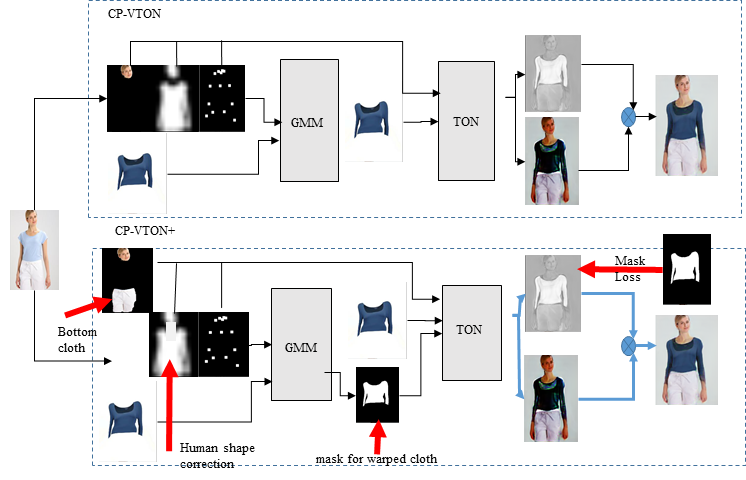
\includegraphics[height=6.5cm, scale=1]{figures/cpvton+pipeline.png}   
\caption{Comparison: CP-VTON and CP-VTON+}
\label{fig:piepline}
\end{figure}